\subsection*{Teil D: Körper und ihre Netze (25 Minuten)}

\begin{enumerate}[resume, label=\arabic*.]
    \item \textbf{Ordne zu - Welches Netz gehört zu welchem Körper?}

    Verbinde mit Linien:

    \begin{center}
        \begin{tabular}{cc}
            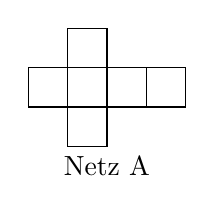
\begin{tikzpicture}[scale=0.5]
                % Würfelnetz
                \draw (0,0) rectangle (1,1);
                \draw (1,0) rectangle (2,1);
                \draw (2,0) rectangle (3,1);
                \draw (3,0) rectangle (4,1);
                \draw (1,1) rectangle (2,2);
                \draw (1,-1) rectangle (2,0);
                \node at (2,-1.5) {Netz A};
            \end{tikzpicture}
            &
            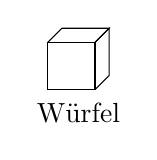
\begin{tikzpicture}[scale=0.6]
                % Würfel
                \draw (0,0) -- (1,0) -- (1,1) -- (0,1) -- cycle;
                \draw (0,1) -- (0.3,1.3) -- (1.3,1.3) -- (1,1);
                \draw (1,1) -- (1.3,1.3) -- (1.3,0.3) -- (1,0);
                \node at (0.65,-0.5) {Würfel};
            \end{tikzpicture}
            \\[2cm]
            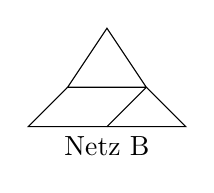
\begin{tikzpicture}[scale=0.5]
                % Pyramidennetz (vereinfacht)
                \draw (0,0) -- (2,0) -- (1,1.5) -- cycle;
                \draw (0,0) -- (-1,-1) -- (1,-1) -- (2,0);
                \draw (2,0) -- (3,-1) -- (1,-1);
                \node at (1,-1.5) {Netz B};
            \end{tikzpicture}
            &
            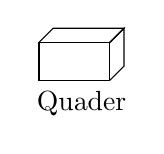
\begin{tikzpicture}[scale=0.6]
                % Quader
                \draw (0,0) -- (1.5,0) -- (1.5,0.8) -- (0,0.8) -- cycle;
                \draw (0,0.8) -- (0.3,1.1) -- (1.8,1.1) -- (1.5,0.8);
                \draw (1.5,0.8) -- (1.8,1.1) -- (1.8,0.3) -- (1.5,0);
                \node at (0.9,-0.5) {Quader};
            \end{tikzpicture}
            \\[2cm]
            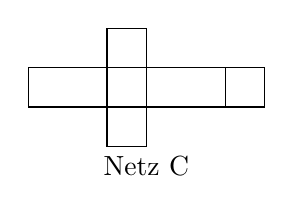
\begin{tikzpicture}[scale=0.5]
                % Quadernetz
                \draw (0,0) rectangle (2,1);
                \draw (2,0) rectangle (3,1);
                \draw (3,0) rectangle (5,1);
                \draw (5,0) rectangle (6,1);
                \draw (2,1) rectangle (3,2);
                \draw (2,-1) rectangle (3,0);
                \node at (3,-1.5) {Netz C};
            \end{tikzpicture}
            &
            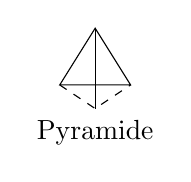
\begin{tikzpicture}[scale=0.6]
                % Pyramide
                \draw (0,0) -- (1.5,0) -- (0.75,1.2) -- cycle;
                \draw[dashed] (0,0) -- (0.75,-0.5) -- (1.5,0);
                \draw (0.75,-0.5) -- (0.75,1.2);
                \node at (0.75,-1) {Pyramide};
            \end{tikzpicture}
        \end{tabular}
    \end{center}

    \vspace{0.5cm}

    \item \textbf{Fülle die Tabelle aus:}

    \begin{center}
        \renewcommand{\arraystretch}{2}
        \begin{tabular}{|l|c|c|c|}
            \hline
            \textbf{Körper} & \textbf{Anzahl Ecken} & \textbf{Anzahl Kanten} & \textbf{Anzahl Flächen} \\
            \hline
            Würfel & & & \\
            \hline
            Quader & & & \\
            \hline
            Pyramide (quadratische Grundfläche) & & & \\
            \hline
        \end{tabular}
    \end{center}

    \vspace{1cm}

    \item \textbf{Oberflächenberechnung:} Ein Würfel hat die Kantenlänge $a = 4$ cm.

    \begin{enumerate}[label=\alph*)]
        \item Wie groß ist eine Seitenfläche? 

        Rechnung: $A_{Seite} = a \cdot a = 4$ cm $\cdot 4$ cm = \underline{\hspace{4cm}}

        \item Wie groß ist die gesamte Oberfläche? 

        Rechnung: $O = 6 \cdot A_{Seite} = 6 \cdot$ \underline{\hspace{2cm}} = \underline{\hspace{3cm}}
    \end{enumerate}

    \vspace{0.5cm}

    \item \textbf{Volumenberechnung:} Ein Quader ist 5 cm lang, 3 cm breit und 2 cm hoch.

    \begin{enumerate}[label=\alph*)]
        \item Berechne das Volumen:

        Rechnung: $V = l \cdot b \cdot h = 5$ cm $\cdot 3$ cm $\cdot 2$ cm = \underline{\hspace{4cm}}

        \item Wie viele Würfel mit 1 cm Kantenlänge passen hinein? 

        Antwort: Es passen \underline{\hspace{3cm}} Einheitswürfel hinein.
    \end{enumerate}
\end{enumerate}
